\chapter{Il Sistema Internazionale e i campioni delle unità di misura}

\begin{figure}[h]
    \centering
    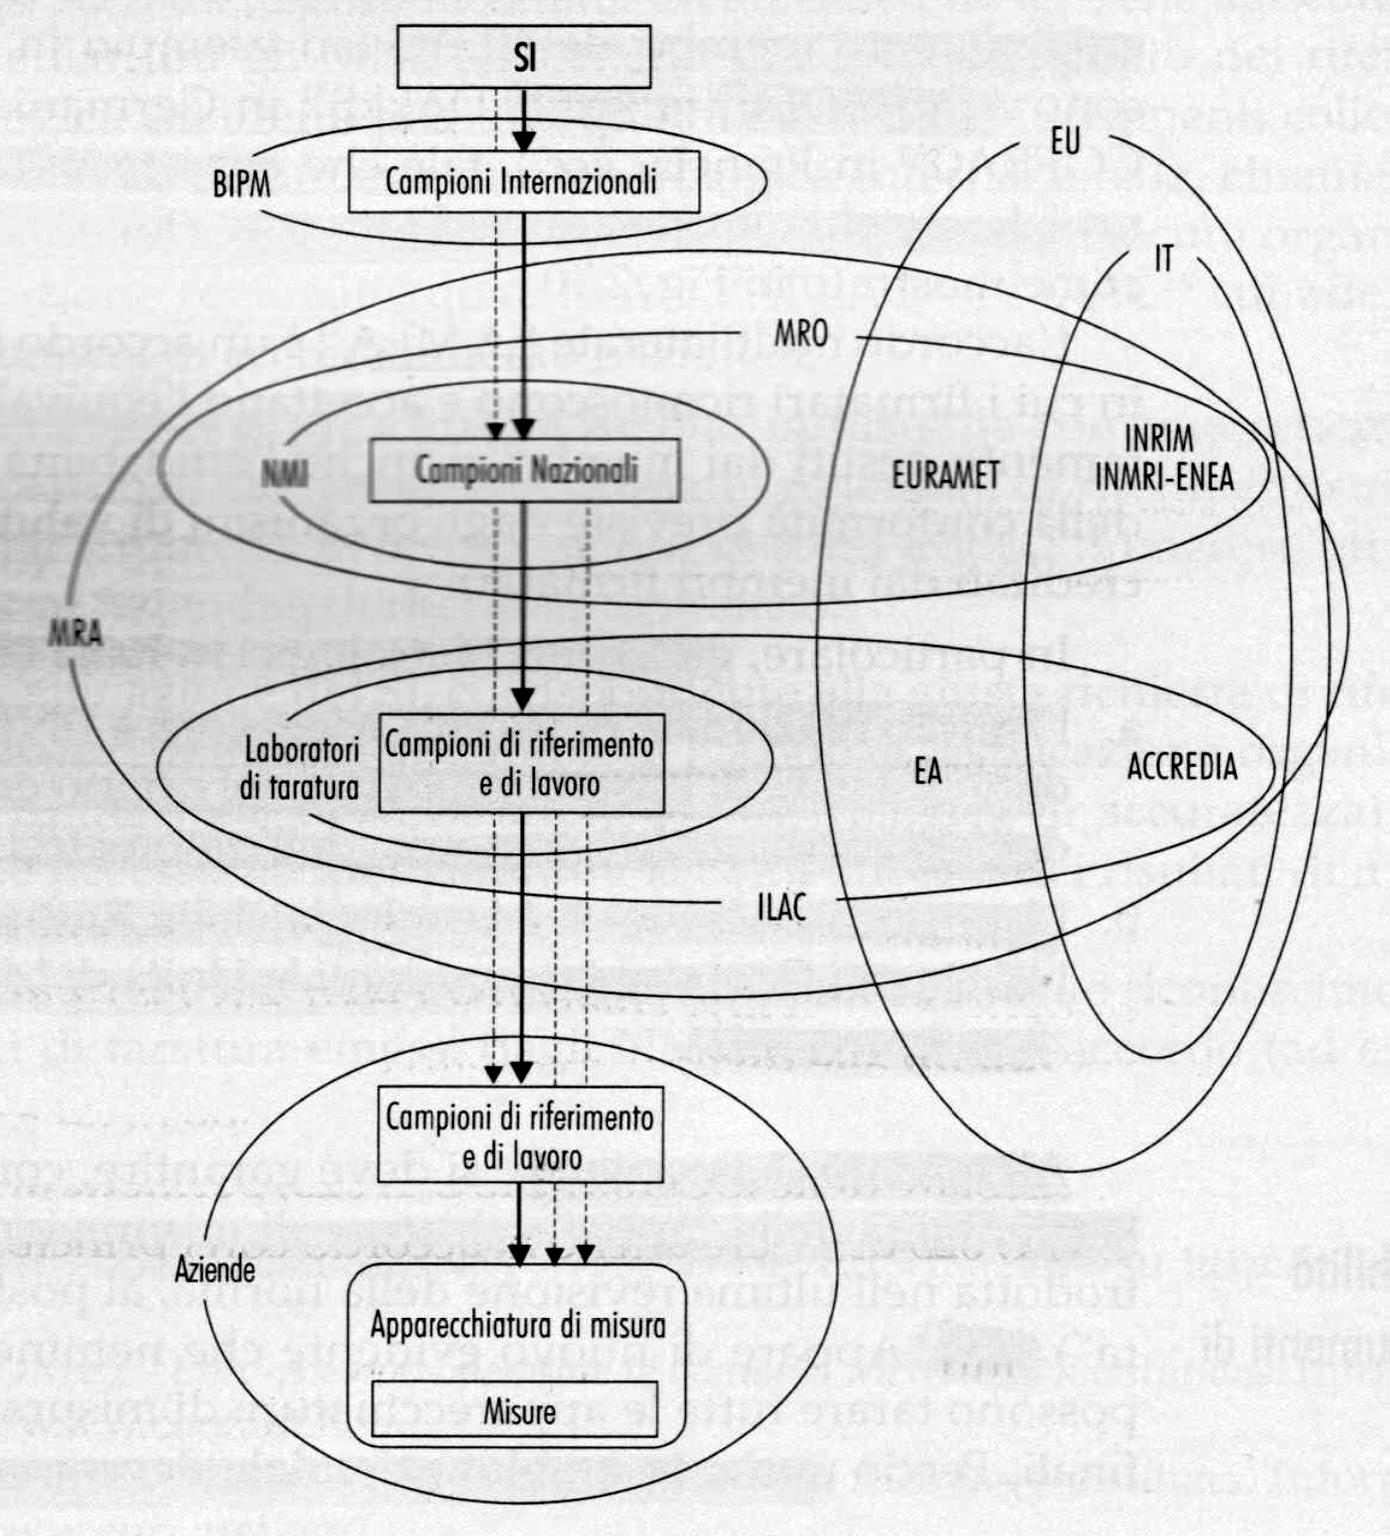
\includegraphics[scale = 0.3]{Disseminazione internazionale dell'SI.png}
\end{figure}

\newpage 

\section{I campioni e la riferibilità delle misure}
\footnote{Slide della prof | SDME 1.4 Metrologia - Riferibilità | pag 2 - 5 \\  
Appunti | 2025-03-04 | pag 6}

L'espressione "riferibilità delle misure" fa riferimento all'allineamento dello strumento 
di misura al corrispondente campione primario (che sta al BIPM). \newline 

La riferibilità è fondamentale tutte le volte che l'operazione di misura viene svolta in modo indipendente da due oggetti distinti. \newline 

\begin{tcolorbox}
    Il concetto di riferibilità è molto teorico, ma è molto importante in fatto di misure, 
    sennò misureremo patate piuttosto che grandezze oggettive
\end{tcolorbox}

Il concetto di riferibilità a coppie e globale lo si può spiegare con il seguente schema: 

\begin{figure}[h]
    \centering
    \includegraphics[scale = 1]{Riferibilità a coppie e globale.png}
\end{figure}

I due cerchi che si trovano sullo stesso piano, 
possono rappresentare due strumenti che hanno una riferibilità a coppia, 
ma che, allo stesso momento, si riferiscono allo strumento di entità maggiore 
(quello rosso). \newline 

Da notare anche le frecce del disegno, che indicano la riferibilità tra i dispositivi di misura. \newline 

Quando vi è una moltitudine di soggetti coinvolti, 
l'armonizzazione a coppie non è possibile: ecco perché risulta necessario un riferimento globale 
rispetto al quale ogni strumento deve essere in armonia. \newline 

Grazie al concetto di riferibilità, 
è possibile esprimere le seguenti proprietà: 

\begin{itemize}
    \item Proprietà distributiva, cioè due strumenti che sono in armonia col riferimento globale risultano in armonia l'uno con l'altro 
    \item Proprietà transitiva, cioè uno strumento, se risulta in armonia con un altro che è in armonia col riferimento globale, è a sua volta in armonia col riferimento globale
\end{itemize}

Un esempio della proprietà transitiva può essere spiegato con il seguente schema: 

\begin{figure}[h]
    \centering
    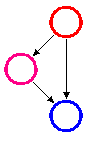
\includegraphics[scale = 1]{Proprietà transitiva della riferibilità.png}
\end{figure}

Per consentire e facilitare la diffusione della riferibilità a livello mondiale, 
è stata istituita una catena della riferibilità che ha una struttura piramidale. \newline 

Alla base di questa catena ci sono, ad esempio in Italia, i centri di "Laboratorio Accreditati di Taratura" o LAT. \newline 

\newpage 

Un esempio di catena di riferibilità: 

\begin{figure}[h]
    \centering
    \includegraphics[scale = 0.3]{Catena di riferibilità.png}
\end{figure}

Un altro esempio di catena di riferibilità per l'Italia: 

\begin{figure}[h]
    \centering
    \includegraphics[scale = 0.3]{Catena di riferibilià Ancona.png}
\end{figure}

Un esempio di catena di riferibilità tra paesi differenti: 

\begin{figure}[h]
    \centering
    \includegraphics[scale = 0.3]{Catena di riferibilià Italia e USA.png}
\end{figure}

Come si può visualizzare, anche se i paesi sono differenti, si garantisce la catena della riferibilità. \newline 

\newpage 

\section{I campioni secondari}
\footnote{Slide della prof | SDME 1.4 Metrologia - Riferibilità | pag 6 - 8 \\  
Appunti | 2025-03-04 | pag 7}

I LAT, per esteso Laboratori Accreditati di Taratura, conservano i campioni secondari distribuiti sul territorio nazionale. \newline 

La disseminazione dei campioni ha lo scopo di facilitare la riferibilità delle misure al campione primario 
(o di riferimento) nazionale. \newline 

Periodicamente, i campioni secondari dei LAT vengono confrontati con il campione nazionale, al fine di garantire la riferibilità. \newline 

Esempi di campioni secondari di f.e.m. e resistenza sono il Fluke 734A e il Fluke 742A.  \newline 

Un altro strumento molto importante nelle misure è il calibratore, 
che è quello strumento che permette di confrontare due grandezze omogenee. \newline 

Un esempio di calibratore è il Fluke 5500A, che ha una fluttuazione di tensione di 50 parti per milione (o ppm) in 1 anno e 
una fluttuazione di resistenza di 90 ppm in 1 anno. \newline 

Non c'è una legge analitica per la calibrazione e la taratura, ma generalmente, 
la fluttuazione indicata in uno strumento viene garantita per un anno dal LAT e/o dal costruttore da cui si è appena acquistato lo strumento di misura. \newline 

\newpage 

\section{Disseminazione internazionale del SI}
\footnote{Slide della prof | SDME 1.4 Metrologia - Riferibilità | pag 20 - 21 \\  
Appunti | 2025-03-04 | pag 11}

Grazie al seguente schema, è possibile rappresentare la disseminazione internazionale dell'SI: 

\begin{figure}[h]
    \centering
    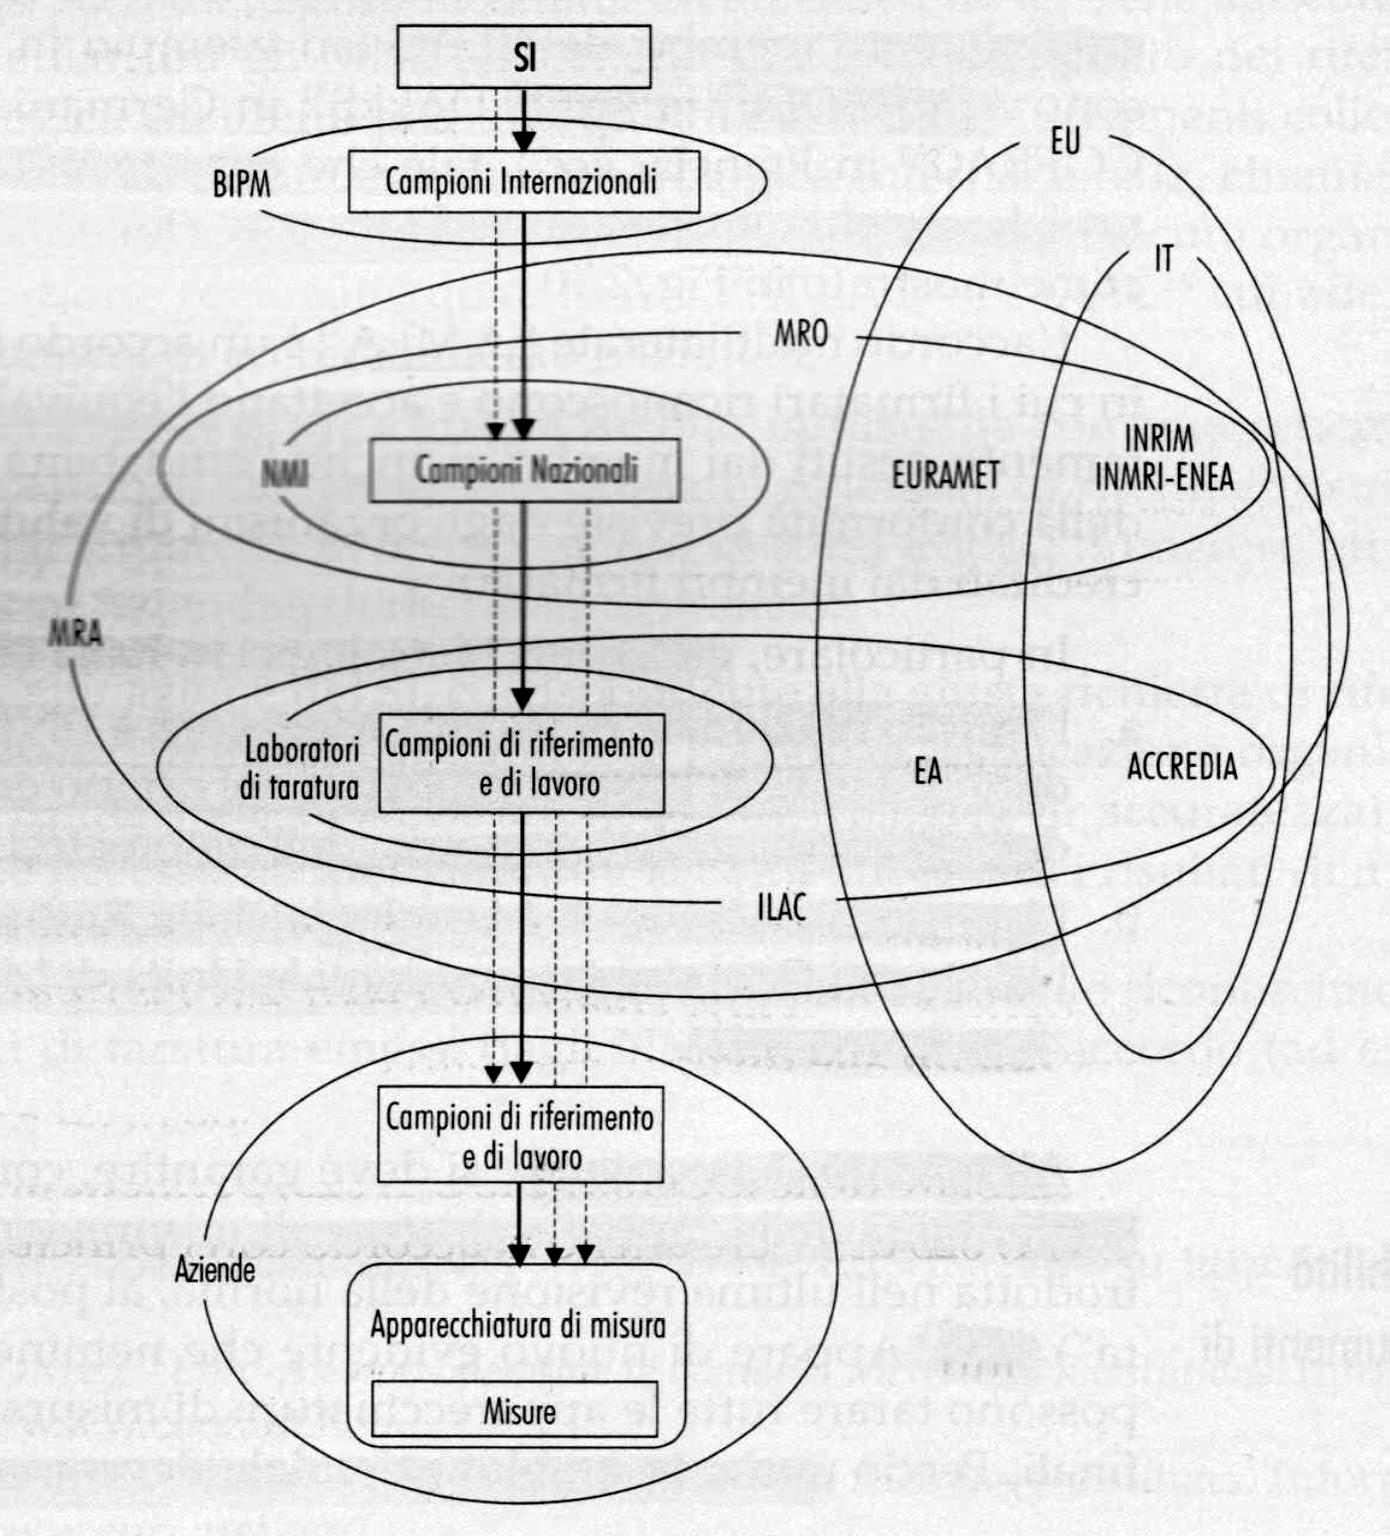
\includegraphics[scale = 0.2]{Disseminazione internazionale dell'SI.png}
\end{figure}

Essendo la catena della riferibilità piramidale, 
andando dall'alto verso il basso, la catena si divide in: 

\begin{itemize}
    \item Primo livello: la convenzione del metro stabilisce l'SI come Sistema Internazionale delle Unità di misura e istituisce il BIPM ed i relativi campioni internazionali 
    \item Secondo livello: gli istituti nazionali di Metrologia (NMI) mantengono e confrontano l'SI e lo rendono disponibile per la disseminazione 
    \item Terzo livello: qui operano i laboratori di taratura accreditati dagli organismi di accreditamento nazionali
    \item Disseminazione in ambito industriale con schema piramidale, i.e. i campioni aziendali vengono utilizzati per tarare gli strumenti di lavoro 
\end{itemize}

Nelle aziende ci possono essere due tipi di strumenti: 

\begin{itemize}
    \item quelli da banco, che generalmente sono pesanti, si trovano nei laboratori e vengono utilizzati per la calibrazione 
    \item quelli da utilizzare sul campo, i quali vengono tarati grazie agli strumenti di misura da banco
\end{itemize}

\newpage 

\section{Campioni per montaggio negli strumenti}
\footnote{Slide della prof | SDME 1.4 Metrologia - Riferibilità | pag 9 - 19}

\subsection{Diodi zener e a valanga}
\footnote{Slide della prof | SDME 1.4 Metrologia - Riferibilità | pag 9-14 \\  
Appunti | 2025-03-04 | pag 7 - 9}

Negli strumenti e/o negli apparecchi che utilizziamo, 
viene impiegato il diodo zener e a valanga come il seguente: 

\begin{figure}[h]
    \centering
    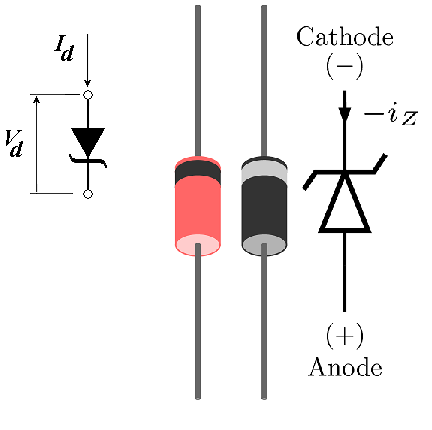
\includegraphics[scale = 0.3]{Diodo zener e schema circuitale.png}
\end{figure}

Una relazione importante nel diodo zener è quella tra tensione a capi di esso e la corrente in uscita, 
come visualizzato nella seguente figura:

\begin{figure}[h]
    \centering
    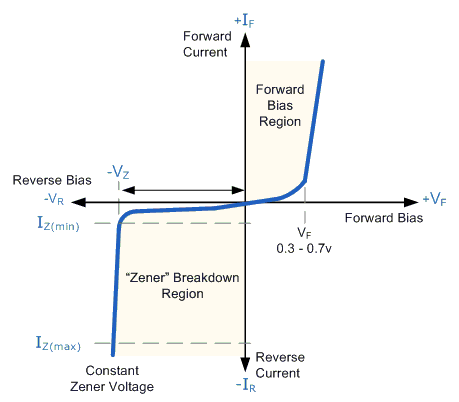
\includegraphics[scale = 0.5]{Relazione tra tensione e corrente in un diodo zener.png}
\end{figure}

Come visualizzato in figura, 
all'aumentare della corrente, la tensione rimane stabile e non si allontana molto da $V_F$, 
che, a secondo del diodo zener, rimane stabile sui $0.3 - 0.7 V$. \newline

Prendendo per esempio una porzione di circuito come il seguente: 

\begin{figure}[h]
    \centering
    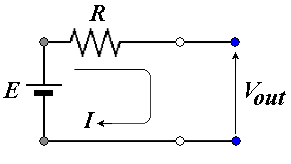
\includegraphics[scale = 0.5]{Circuito generatore di tensione e resistore.png}
\end{figure}

composto da generatore di tensione e resistore. \newline

La corrente che scorre nel circuito è la seguente: 

{
    \Large 
    \begin{equation}
        I = \frac{E}{R} - \frac{V_{out}}{R}
    \end{equation}
}

quindi $V_{out}$ sarà, con semplici sostituzioni:

{
    \Large 
    \begin{equation}
        V_{out} = E - RI
    \end{equation}
}

$V_{out}$ è una funzione della temperatura, della tensione del generatore di tensione E, 
della corrente sulla resistenza I e del tempo, oppure, 
in una formula compatta, possiamo scrivere: 

{
    \Large 
    \begin{equation}
        V_{out} = f(\theta, E, I, t)
    \end{equation}
}

Al variare di E, $V_{out}$ varierà in questo modo: 

\begin{figure}[h]
    \centering
    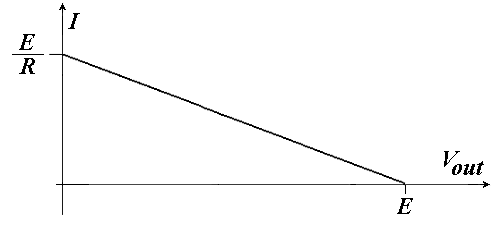
\includegraphics[scale = 0.5]{Circuito generatore di tensione e resistore V out.png}
\end{figure}

Ciò è possibile perché $V_{out}$ è una relazione lineare. \newline

Invece, aggiungendo un elemento non lineare il diodo zener al circuito: 

\begin{figure}[h]
    \centering
    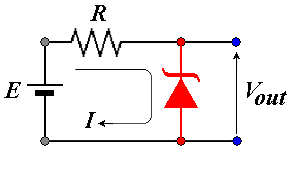
\includegraphics[scale = 0.8]{Circuito generatore di tensione e resistore con diodo zenerpng.png}
\end{figure}

Grazie all'introduzione del diodo zener, quindi di un circuito non lineare, 
la relazione tra tensione di uscita e corrente nel circuito: 

\begin{figure}[h]
    \centering
    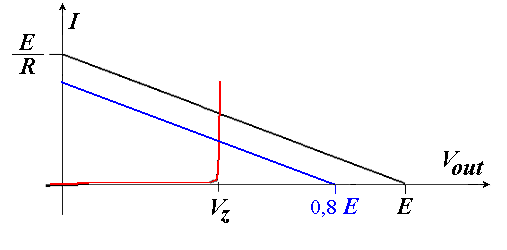
\includegraphics[scale = 0.8]{Relazione tra tensione e corrente con un diodo zener.png}
\end{figure}

Come si può notare dal grafico, 
la corrente deve essere adeguata per ottenere $V_z$, 
ma non eccessiva per non bruciare il diodo zener. \newline 

Inoltre, va calcolata tenendo conto del massimo valore della tensione in ingresso. \newline 

$V_{out}$ è una funzione anche della temperatura perché lo zener soffre di deriva termica. \newline 

Per deriva, si intende che il valore della tensione (e /o di altri parametri), 
cambiano. \newline 

Per deriva termica, in questo caso, si intende che il valore della tensione varia in base alla temperatura $\theta$. \newline 

Sapendo che $V_d$ è la tensione ai capi dello zener e $I_d$ la corrente che circola sullo zener: 

\begin{figure}[h]
    \centering
    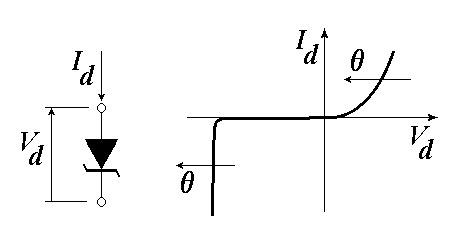
\includegraphics[scale = 0.8]{Diodo zener e drift.png}
\end{figure}

\newpage 

Dalla figura si può notare che la temperatura $\theta$ varia la pendenza della curva. \newline

La deriva termica (o in inglese drift) va scelta in base all'ordine di grandezza della misura che si vuole fare. \newline 

Diamo per esempio due zener con $V_z$ dai 2 ai 70 V: 

\begin{itemize}
    \item il primo è uno zener non compensato che ha un drift di $\pm 1000 ppm/^{\circ} C$ e il suo costo è di $0.02$ Euro 
    \item il secondo è uno zener compensato che un drift di $\pm 10 ppm/^{\circ} C$ e costa 7 Euro
\end{itemize}

Per compensare si intende compensare la temperatura in modo da rendere più stabile il componente. \newline 

Come campioni di f.e.m. negli strumenti vengono utilizzati degli integrati, 
come ad esempio nell'intergrato di regolatore di tensione LM7812 è presente nel circuito uno 
stabilizzatore di tensione, con l'utilizzo di diodi zener. \newline 

LM7812 ha un costo di 70 centesimi di Euro. \newline 

Invece, l'AD587 è un integrato che ha un costo di $21.75$ Euro ed ha un drift minore rispetto all'esempio precedente. \newline 

\newpage 

\subsection{Campioni di resistenza} 
\footnote{Slide della prof | SDME 1.4 Metrologia - Riferibilità | pag 15 - 16 \\  
Appunti | 2025-03-04 | pag 9 - 10 | 2025-06-23 Ricevimento | pag 1 - 2}

Un elemento utilizzato comunemente come campione di resistenza negli strumenti è il resistore a strato a pellicola di carbonio 
come quello in figura: 

\begin{figure}[h]
    \centering
    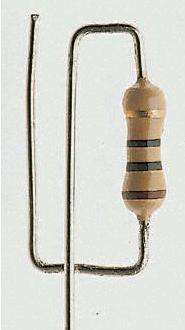
\includegraphics[scale = 0.5]{Resistore a pellicola di carbonio.png}
\end{figure}

Sono i resistori che vengono comunemente utilizzati: 
hanno un basso costo di vendita (generalmente dai 3 ai 6 centesimi). \newline 

L'eccellente stabilità con diverse condizioni di carico o livelli di umidità, 
il livello di rumore ridotto e l'elevata affidabilità, rendono questi resistori a strato di carbone 
adatti ad un'ampia gamma di applicazioni. \newline 

Un esempio di specifiche tecniche per  un resistore a pellicola di carbonio: 

\begin{itemize}
    \item Tolleranza resistenza: $\pm 5 \%$ 
    \item Coefficiente termico da -150 a -850 $\frac{ppm}{^{\circ} C}$ 
    \item Dissipazione di $0.66 W$ a $70 ^{\circ} C$
\end{itemize}

La tolleranza di resistenza e il coefficiente termico sono troppo elevati per una misura. \newline

Inoltre, sono comunemente utilizzati anche perché il valore della resistenza e della sua tolleranza sono definiti 
attraverso un codice a colori sulla resistenza stessa. \newline 

La costruzione fisica del resistore ne influisce il suo comportamento in base alla frequenza 
(cioè il resistore può "diventare" un condensatore e/o un induttore). \newline 

Nel caso di resistore a pellicola di carbonio, il resistore, ad alta frequenza, può avere un comportamento capacitivo. \newline 

Invece, per i resistori ad alta precisione come nel seguente caso: 

\begin{figure}[h]
    \centering
    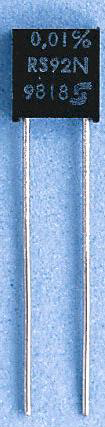
\includegraphics[scale = 0.5]{Resistore ad alta precisione.png}
\end{figure}

hanno una natura di tipo induttivo. \newline 

Da un punto di vista fisico, 
i resistori di precisione sono di metallo massiccio ad altissima stabilità e precisione. \newline 

Inoltre, hanno un bassissimo coefficiente di temperatura, quindi un drift molto basso. \newline 

Un esempio di specifiche tecniche per un resistore di precisione: 

\begin{itemize}
    \item Tolleranza resistenza $\pm 0.01 \% $ 
    \item Coefficiente di temperatura $\pm 5 ppm / ^{\circ} C$ 
    \item Costante di tempo di $1 \cdot 10^{-9}$ s 
    \item Potenza dissipata di $70 ^{\circ} C$ a $0.6 W$
    \item Costo dai 13 ai 23 Euro
\end{itemize}

La costante di tempo del resistore reale è dovuta al fatto che 
il componente reale non si comporta come resistore ideale: 
dato un segnale che ha frequenza oltre alla frequenza di taglio, che è l'inverso della costante di tempo del componente, 
in ingresso al resistore reale,    
questo ultimo ha un comportamento capacitivo. \newline 

In altre parole, il resistore reale si comporta da filtro passa basso 
dato un segnale con frequenza maggiore dell'inverso della costante di tempo. \newline 

Il resistore di precisione di metallo massiccio ha un comportamento capacitivo perchè è realizzato compremendo un filo in modo molto fitto, 
e ciò rende l'interno di un resistore come il dielettrico di un condensatore. \newline 

\newpage 

\subsection{Campioni di tempo}
\footnote{Slide della prof | SDME 1.4 Metrologia - Riferibilità | pag 17 - 19 \\  
Appunti | 2025-03-04 | pag 10 - 11}

Il tempo è la grandezza fisica che riusciamo a misurare meglio, con più precisione. \newline 

All'interno degli strumenti, un circuito comunemente utilizzato per temporizzare il tempo 
è quello di un oscillatore con rete RC come in figura: 

\begin{figure}[h]
    \centering
    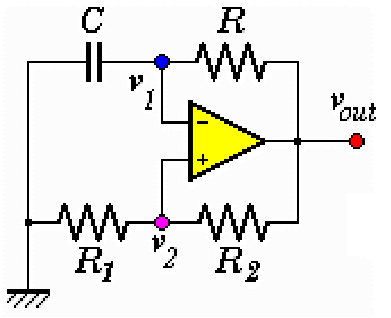
\includegraphics[scale = 0.5]{Oscillatore RC.png}
\end{figure}

Il periodo di oscillazione è proporzionale a RC. \newline 

Un problema di questo circuito è quello che, se non viene compensato, 
il circuito è fortemente influenzato dalla temperatura, in particolare i valori di R e di C. \newline 

La regola generale è che, se ci sono più componenti in circuito, ogni componente causa una deriva e, nel complesso, 
le derive si sommano. \newline 

Un altro elemento fisico impiegato nei circuiti per campionare il tempo è quello del quarzo. \newline 

La proprietà del quarzo è quello di avere un effetto piezoelettrico, 
cioè che ad un effetto meccanico influisce poi un effetto elettrico. \newline 

L'effetto piezoelettrico può essere utilizzato per pilotare un circuito elettrico, 
in grado di portare e mantenere in oscillazione il quarzo, reintegrando ad ogni oscillazione l'energia dissipata della deformazione elastica. \newline 

I cristalli di quarzo come in figura: 

\begin{figure}[h]
    \centering
    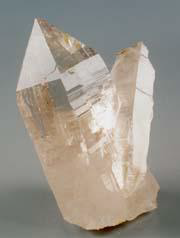
\includegraphics[scale = 0.5]{Cristallo di quarzo.png}
\end{figure}

hanno le seguenti caratteristiche tecniche: 

\begin{itemize}
    \item sono disponibili con diverse frequenze nominali: da 32.768 kHz ad altro 30 MHz 
    \item sono stabili 
    \item sono economici: dai 50 centesimi ai circa 3 Euro
\end{itemize}

ma, il più grande problema, è che necessitano di componenti supplementari. \newline 

Allora, possono essere utilizzati altri componenti per campionare il tempo, 
ad esempio un TCXO (Temperature-compensated crystal oscillator). \newline 

Un TXCO è autonomo, economico, stabile, ma, a seconda del modello, richiedere un tempo non trascurabile per stabilizzarsi. \newline 

\newpage 





